% reducesymm/blog/dailyBlogKS.tex
% Predrag  created              Sep 2 2013
% continues siminos/blog/dailyBlog.tex as of that date

\chapter{Kamal's daily blog}
\label{c-dailyBlogKS}

\begin{description}
\item[2013-07-11  Predrag to Kamal] Created this for you to blog
in. Burak will show you the ropes. You need to register on gitHub, let me
know your user ID there.

\item[2013-10-15  Kamal] I am working on symmetry reduction in spiral waves and have studied a few research papers by Barkley, Biktashev. I am trying to find out how to start working on the problem. In the 1994 paper by Barkley and Kevrekidis {\em A dynamical systems approach to spiral waves dynamics} and another paper by Barkley (Phys. Rev. Lett. 72, 1994), they have given an equivalent system of ODE in place of the actual Reaction-Diffusion PDEs. These ODEs also have time shift and $E(2)$ symmetry. Should I apply symmetry reduction on these ODEs or begin with the PDEs?

\item[2013-10-15 Predrag] Our main conceptual confusion (with none of us having
done any actual work so far) is how rotations and translations interact - \ie, if you change the origin and then translate is different from first translating and then rotating. I think you can figure out how that really works in the Barkley ODE system first - that would be a great help. My intuition (usually wrong) is that we want to
quotient the rotational $\SOn{2}$ first.

\item[2013-10-12  Kamal] I will be away during the month of January for my wedding.
I will be working from home and updating through GitHub.
Please let me know if you have anything you want me to take care of.
Further, it will be great for me if you could send me the material
for the QFT final project. As you might have experienced, speed is
an issue with my working on new stuff so I want to start as early
as possible to get something useful out of it given the time constraints.
Also the TA duties are killing me. I am working on it and want to be productive fast.

\item[2013-10-17 Predrag] I was thinking that it might be useful to
learn about the \emph{`Gribov ambiguity'}.
What follows are some of my notes from
svn repository
\\
\texttt{siminos/blog/lit.tex}. Have a look...

\item[2012-05-20 Jeff Greensite] has written a book\rf{Greensite11} of
possible interest, \emph{An introduction to the confinement problem}.

\HREF{http://en.wikipedia.org/wiki/Gribov_ambiguity}{Gribov ambiguity wiki}
(edits by Predrag):

Gauge fixing means choosing a representative from each gauge orbit. The
space of representatives is a submanifold and represents the gauge fixing
condition. Ideally, every gauge orbit will intersect this submanifold
once and only once. This is generally impossible globally, especially for
non-abelian gauge theories, because of topological obstructions and the
best that can be done is make this condition true locally. A gauge fixing
submanifold may not intersect a gauge orbit at all or it may intersect it
more than once. This is called a Gribov\rf{Gribov77} ambiguity.

Gribov ambiguities lead to a nonperturbative failure of the BRST
symmetry, among other things.

A way to resolve the problem of Gribov ambiguity is to restrict the
relevant functional integrals to a single \emph{Gribov region} or {\em
fundamental modular region} whose boundary is called a \emph{Gribov
horizon}.

{\em Gribov copies} play a crucial role in the infrared (IR) regime while
it can be neglected in the perturbative ultraviolet (UV)
regime\rf{Gribov77,Zwanz89,Zwanz93}. The restriction to the Gribov region
(defined in such a way that the Faddeev-Popov operator is strictly
positive) can be achieved by adding a nonlocal term, commonly known as
`horizon term', to the YM action\rf{Zwanz89,Zwanz93,Zwanz92}. This is a
nonlocal term in the 4-dimensional Euclidean space, written as an
integral over the `horizon function.'

Greensite: ``In non-Abelian theories, there are many gauge copies -
Gribov copies - that satisfy the Coulomb gauge condition. The Gribov
region is the space of all Gribov copies with positive Faddeev-Popov
eigenvalues. Configurations of the Gribov horizon have at least one FP
eigenvalue $\lambda =0$. What counts for confinement is the density of
eigenvalues $\rho(\lambda)$ near $\lambda =0$, and the `smoothness' of
these near-zero eigenvalues.

The Gribov horizon is a convex manifold in the space of gauge fields,
both in the continuum and on the lattice. The Gribov region, bounded by
that manifold, is compact.
''

Amusingly, they can find the first 200 eigenstates of the lattice
Faddeev-Popov operator on each time-slice of each lattice configuration
by the Arnoldi algorithm.

See also Heinzl\rf{Heinzl96,HeRuSch08}, as well as
\refrefs{RuSchVo02,MaScha94,vanBaal91,DellAnZwan91,Cutkosky84,Singer78}.
Review of \refref{VaZw12} promises ``to give a pedagogic review of the
ideas of Gribov and the subsequent construction of the GZ action,
including many other topics related to the Gribov region.''

Nele Vandersickel
\HREF{http://physik.uni-graz.at/~dk-user/talks/Vandersickel20100225.pdf}
{talk} gives a compact overview, might be useful for writing this up.
Chapter 3 of her thesis, \arXiv{1104.1315}, gives a pedagogic overview of
the Gribov-Zwanziger framework, not available yet in the literature.

\item[2012-06-14 Predrag]
\HREF{http://marcofrasca.wordpress.com/about/}{Frasca} is either insane
or just yet another ignorant field theorist: ``I have worked on almost
all fields of physics'' (???). I checked the publication list, and it is
no  L.D. Landau. But the blog is informative:

{\bf [2012-06-05 Frasca]} (edited by Predrag):

``The answer to the question of the mass gap in Yang-Mills theory has
made enormous progress mostly by the use of lattice computations and,
quite recently, with the support of theoretical analysis. Contrarily to
common wisdom, the most fruitful attack to this problem is using Green
functions. The reason why this was not a greatly appreciated approach
relies on the fact that Green functions are gauge dependent.
Nevertheless, they contain physical information that is gauge independent
and this is exactly what we are looking for: The mass gap.''

(Predrag: this I interpret in the spirit of Gutzwiller - the Green function
is coordinate dependent, but it's trace - which yield the spectrum - is
coordinate invariant.)

``\HREF{http://marcofrasca.wordpress.com/2011/01/28/the-saga-of-landau-gauge-progators-a-short-history/}
{The Saga of Landau-Gauge Propagators: A Short History}'' is a good read:

``We cannot forever ignore the low energy behavior of QCD as its complete
understanding could have impact at unexpected large scales.''

\item[2012-06-15 Predrag]
Laufer and Orland\rf{LauOrl12} say in
{\em The geometry of {Yang-Mills} orbit space on the lattice}: ``
We find coordinates, the metric tensor, the inverse metric tensor and the
Laplace-Beltrami operator for the orbit space of Hamiltonian SU(2) gauge
theory on a finite, rectangular lattice. This is done using a complete
axial gauge fixing. The Gribov problem can be completely solved, with no
remaining gauge ambiguities.
''

\item[2012-06-15 Evangelos]
This seems very interesting and I have to read it. It will most probably
confuse people, if we are really addressing fluid-dynamicists.

{\bf [2012-06-15 Predrag]} I am trying to reach out to quantum filed
theorists, that's why these facts are made explicit here - otherwise they
think it is just plumbing, nothing to do with Fundamental Physics..

Maybe shorten it? For instance Faddeev-Popov operator is not introduced
here, so we might avoid reference to it altogether. In the last sentence,
is the Gribov region or the Gribov horizon a convex manifold?

{\bf [2012-06-15 Predrag]} Better now? {\bf [2012-06-15 Evangelos]}  Yes.
Something that still confuses me: Is `Faddeev-Popov operator' really the
gauge orbit tangent vector, or is it the group generator? {\bf
[2012-06-15 Predrag]} I think `group generator' would not have enough
information (why should it be position dependent?), so it should be
something like our group orbit tangent vector, except positivity of
eigenvalues sounds like a projection on a given direction across the
slice. Do not now yet, so I toned it down in the text.

\item[2013-10-17 Predrag] The above posts summarize all my
notes about the \emph{`Gribov ambiguity'}. I fear it is way too difficult,
starting with Kamal's current background in QFT, but it is one of
directions in which our current symmetry-reduction work might
develop in the future...

\item[2013-10-19 Kamal to Predrag] I tried to reduce \SOn{2} symmetry
from the dynamics of the system of five nonlinear ODEs proposed by
Barkley and Kevrekidis\rf{BarKev94}:
\bea
\dot{x} &=& s \cos{\phi} \,,\qquad
\dot{y} = s \sin{\phi}\,,\qquad
\dot{\phi} =  w \, h(s^2,w^2)     \continue
\dot{s}  &=& s \, f(s^2,w^2) \,,\qquad
\dot{w}= w \, g(s^2,w^2)
\,.
\label{BarKev94-6}
\eea
$(x,y)$ is the position of the spiral tip, $s$ is the tip speed, and
$\dot{\phi}= \gamma_0 w$ the instantaneous rotational frequency. The
dynamics of a spiral are independent of its position.

The group orbits corresponding to \SOn{2} are non-compact in this
case and form counter-clockwise helices, due to which there is an
infinite number of intersections between a particular group orbit and
the slice. As we discussed, I found the intersection of group orbit
of each point on the original trajectory with the slice which is
closest to the template point. Now the problem is I am getting
discontinuous curves as group orbits.

\begin{figure}[b]
\begin{center}
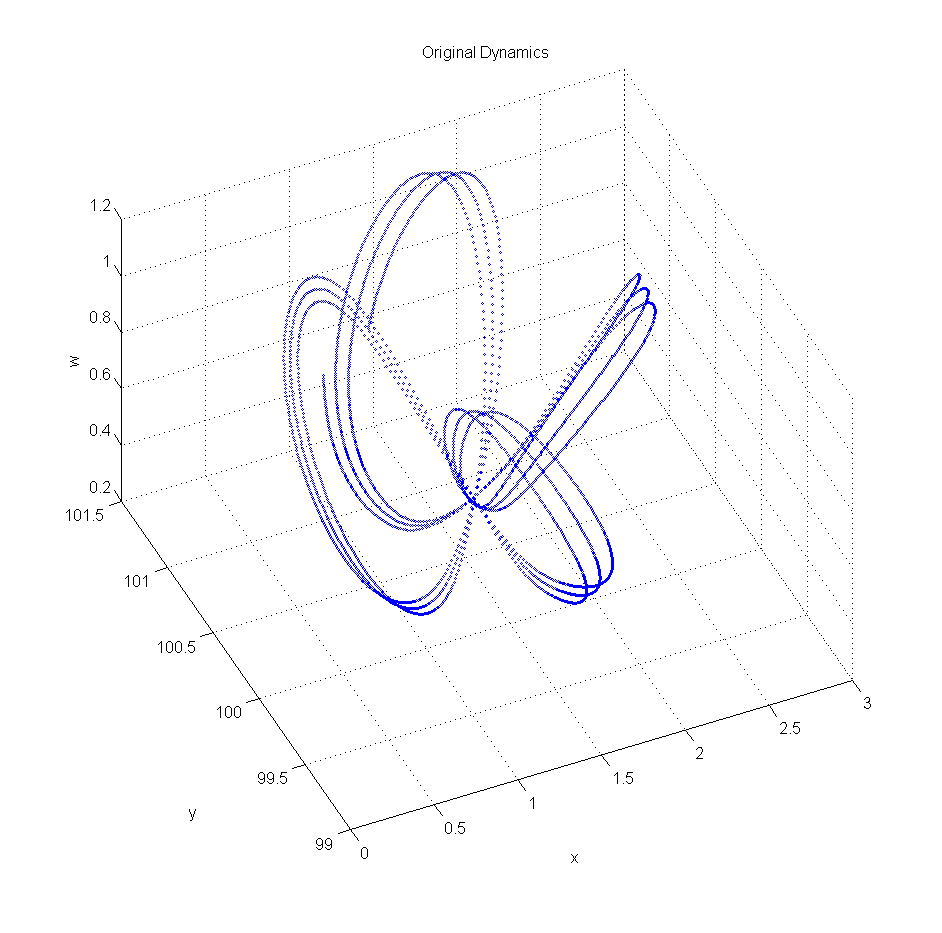
\includegraphics[width=0.5\textwidth]{ksk_spiral2}
\end{center}
\caption{ Trajectory in the full \statesp\ projected on $(x,y,w)$.
    }
\label{fig:ksk_spiral2}
\end{figure}

\begin{figure}[ht]
\begin{center}
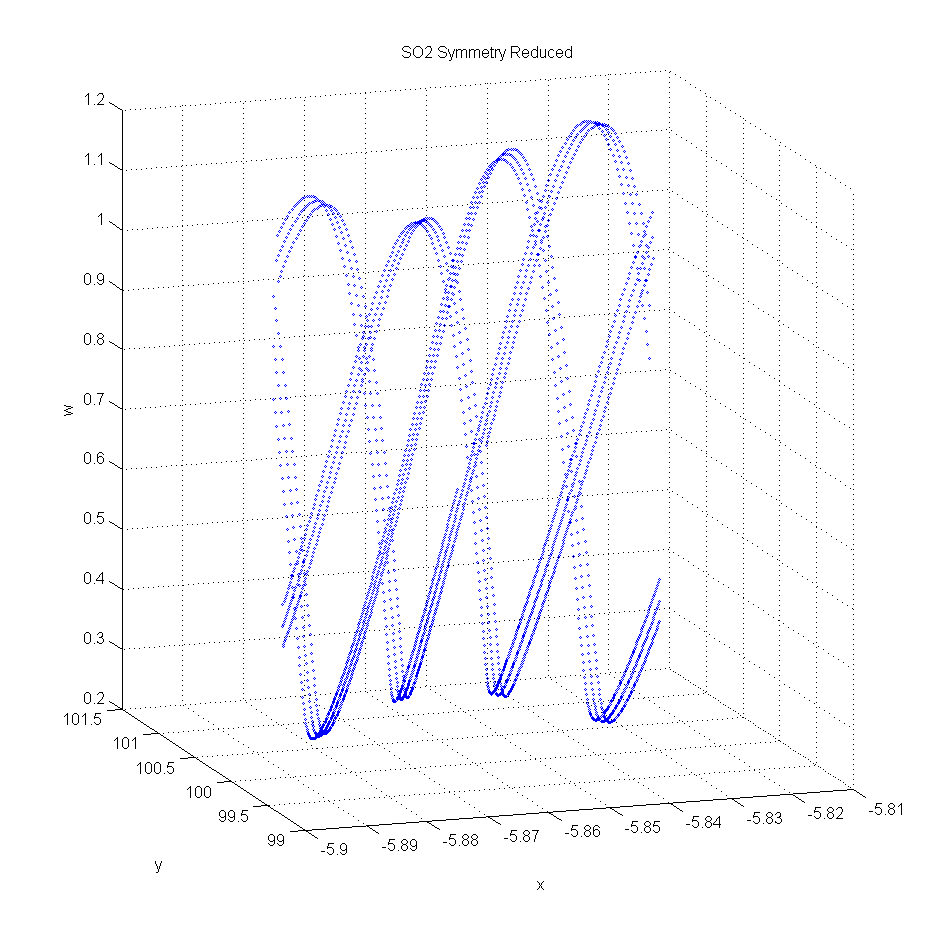
\includegraphics[width=0.5\textwidth]{ksk_so2_w}
\end{center}
\caption{ Reduced \statesp\ dynamics projected on (x,y,w).
    }
\label{fig:ksk_so2_w}
\end{figure}

I am guessing this because I don't have a clever way to find
continuous orbits or because I haven't removed the translational
symmetry yet. Which brings me to the question, how do I remove
translational symmetry? From what I understand since the system is
translationally invariant, I can identify all the points on the plane
to the origin. But this is too trivial or/and too extreme. This
however still doesn't give me a \rpo.
Kindly suggest something.
%\textit{Excuse the format of figures. Still learning LATEX.}

\item[2013-10-20 Predrag] At the moment I have nothing insightful to add,
but Barkley and Kevrekidis\rf{BarKev94} seems to be well written, worth
understanding. My claim is that after symmetry reduction, the dynamics is
(5-1-2) = 2\dmn, so the solutions are either \eqva, circles, or infinite
lines, reconstruction equations yield all regular motions in
their Fig.~4, that's why there is no chaos in the 5\dmn\ ODEs.

\item[2013-10-20 Predrag] Our method of slices is based on the idea that
we look for the point on group orbit of the state $\ssp$ that is closest
to our template. I do not know whether this is a helpful remark, but
i think that is the same as the method of finding a
\HREF{https://inst.eecs.berkeley.edu/~ee127a/book/login/l_svd_lineqs.html}
{pseudo-inverse}.

\item[2013-10-20 Predrag] You might find Saldana's blog of interest, he
has read much of the literature you study in detail; it is
in the svn repository \emph{DOGS}. Your svn ID is \emph{ksharma4},
password \emph{slice!} - Burak or Chris can help you check the repository
out.


\end{description}
\renewcommand{\ssp}{a}
